\section{Resultados}

% \textcolor{red}{Que fue lo que se logró con la experimentación, incluir tablas y parámetros, gráficos (por ejm boxplot), lo más explicativo posible. En los resultados se espera que concluya cuál fue el rendimiento del algoritmo con los experimentos detallados en la sección anterior, y compare las diferencias entre configuraciones distintas de los experimentos. Analizar los resultados obtenidos y concluir acerca de aspectos del algoritmo y/o de la complejidad de las instancias, o acerca de características relacionadas con su implementación.}

A continuación se peresentan los mejores resultados obtenidos con cada una de las instancias. Todas fueron ejecutadas con un $K=1000$, pero ninguna requirió de todas esas iteraciones.

El formato de salida es el siguiente:

\begin{itemize}
    \item Primera línea: 
    \begin{itemize}
        \item Calidad de la solución.
        \item Costos totales del transporte.
        \item Ganancia bruta según el tipo de leche.
    \end{itemize}
    \item $N$ líneas que muestran la información de las $N$ rutas que fueron asignadas a los camiones (mostradas según el orden de los camiones).
    \begin{itemize}
        \item Granjas asignadas a esta ruta, en el orden en el que se deben recorrer. También se muestra al inicio y al final el nodo correspondiente a la planta procesadora.
        \item Costo de transporte de esta ruta.
        \item Cantidad de leche transportada en esta ruta.
        \item Calidad de la leche resultante.
    \end{itemize}
    \item Finalmente, se muestra el tiempo total de la ejecución, medido en milisegundos.
\end{itemize}

\begin{center}
    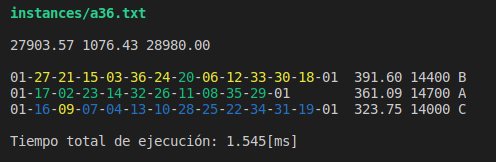
\includegraphics[width=\columnwidth]{imagenes/a36}
\end{center}
\begin{center}
    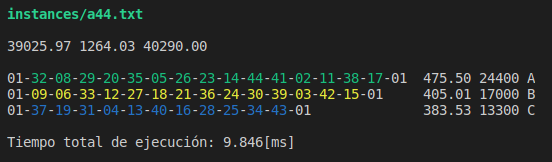
\includegraphics[width=\columnwidth]{imagenes/a44}
\end{center}
\begin{center}
    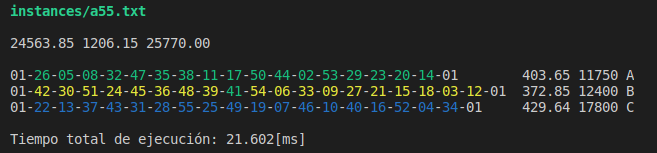
\includegraphics[width=\columnwidth]{imagenes/a55}
\end{center}
\begin{center}
    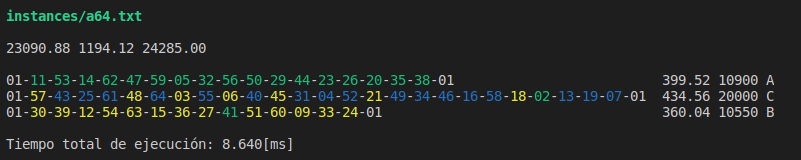
\includegraphics[width=\columnwidth]{imagenes/a64}
\end{center}
\begin{center}
    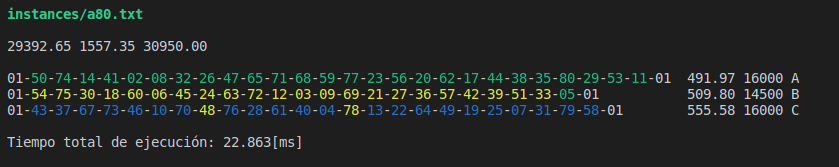
\includegraphics[width=\columnwidth]{imagenes/a80}
\end{center}
\begin{center}
    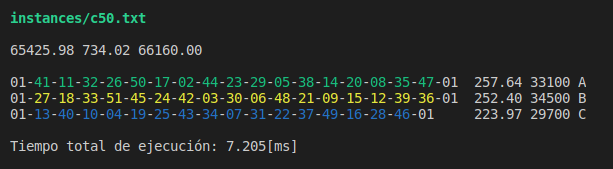
\includegraphics[width=\columnwidth]{imagenes/c50}
\end{center}
\begin{center}
    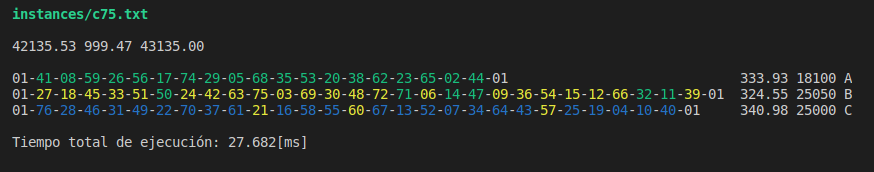
\includegraphics[width=\columnwidth]{imagenes/c75}
\end{center}
\begin{center}
    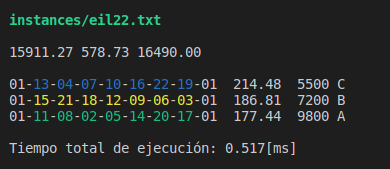
\includegraphics[width=\columnwidth]{imagenes/eil22}
\end{center}
\begin{center}
    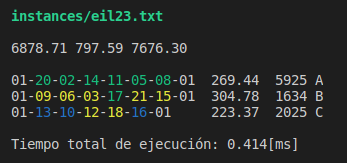
\includegraphics[width=\columnwidth]{imagenes/eil23}
\end{center}
\begin{center}
    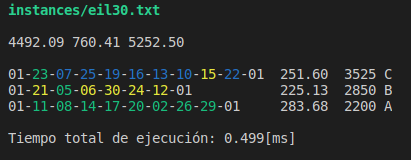
\includegraphics[width=\columnwidth]{imagenes/eil30}
\end{center}
\begin{center}
    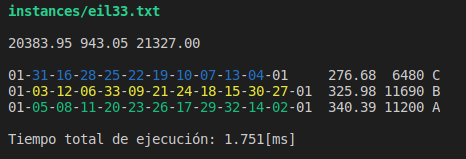
\includegraphics[width=\columnwidth]{imagenes/eil33}
\end{center}
\begin{center}
    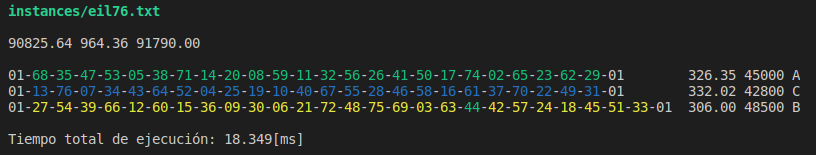
\includegraphics[width=\columnwidth]{imagenes/eil76}
\end{center}

